% !TEX TS-program = pdflatex
% !TEX encoding = UTF-8 Unicode

% This is a simple template for a LaTeX document using the "article" class.
% See "book", "report", "letter" for other types of document.

\documentclass[11pt]{report} % use larger type; default would be 10pt

\usepackage[utf8]{inputenc} % set input encoding (not needed with XeLaTeX)

%%% Examples of Article customizations
% These packages are optional, depending whether you want the features they provide.
% See the LaTeX Companion or other references for full information.

%%% PAGE DIMENSIONS
\usepackage{geometry} % to change the page dimensions
\geometry{a4paper} % or letterpaper (US) or a5paper or....
% \geometry{margin=2in} % for example, change the margins to 2 inches all round
% \geometry{landscape} % set up the page for landscape
%   read geometry.pdf for detailed page layout information

\usepackage{graphicx} % support the \includegraphics command and options

% \usepackage[parfill]{parskip} % Activate to begin paragraphs with an empty line rather than an indent

%%% PACKAGES
\usepackage[english,swedish]{babel}
\usepackage{booktabs} % for much better looking tables
\usepackage{array} % for better arrays (eg matrices) in maths
\usepackage{paralist} % very flexible & customisable lists (eg. enumerate/itemize, etc.)
\usepackage{verbatim} % adds environment for commenting out blocks of text & for better verbatim
\usepackage{subfig} % make it possible to include more than one captioned figure/table in a single float
% These packages are all incorporated in the memoir class to one degree or another...

%%% HEADERS & FOOTERS
\usepackage{fancyhdr} % This should be set AFTER setting up the page geometry
\pagestyle{fancy} % options: empty , plain , fancy
\renewcommand{\headrulewidth}{0pt} % customise the layout...
\lhead{}\chead{}\rhead{}
\lfoot{}\cfoot{\thepage}\rfoot{}

%%% SECTION TITLE APPEARANCE
\usepackage{sectsty}
\allsectionsfont{\sffamily\mdseries\upshape} % (See the fntguide.pdf for font help)
% (This matches ConTeXt defaults)

%%% ToC (table of contents) APPEARANCE
\usepackage[nottoc,notlof,notlot]{tocbibind} % Put the bibliography in the ToC
\usepackage[titles,subfigure]{tocloft} % Alter the style of the Table of Contents
\renewcommand{\cftsecfont}{\rmfamily\mdseries\upshape}
\renewcommand{\cftsecpagefont}{\rmfamily\mdseries\upshape} % No bold!

%Set graphics path
\graphicspath{ {img/} }

%add references and setup biblatex
% setup biblatex/bibliography

%%% END Article customizations

%%% The "real" document content comes below...

\title{Towards impressive titles}
\author{Tobias Axelsson}
%\date{} % Activate to display a given date or no date (if empty),
         % otherwise the current date is printed 

\begin{document}
\maketitle

\chapter*{Acknowledgements}
	\thispagestyle{empty}
	I am a student blalsadf

\selectlanguage{english}
\begin{abstract}
	asdasd
\end{abstract}

\selectlanguage{swedish}
\begin{abstract}
	asdasdasd
\end{abstract}
\selectlanguage{english}

\tableofcontents
	\thispagestyle{empty}


\chapter{Introduction}
\emph{The chapter starts with a background describing why road condition monitoring is important and who Trafikverket are, how road condition data is collected today and why the technology behind it needs improvement. Later on, machine learning basics are explained and how it can be used in this project. An objective for the project is defined followed by its delimitations. Lastly, a thesis structure is presented to simplify navigation through different parts of the project.}

\section{Background} \label{sec:background}
	Living in cold areas of the world usually means work for invididual people, municipalities and companies in trying to maintain a non-winter-like infrastructure. This of course, also involves winter road maintenance. Salting and plowing roads is an investment in not only saving lives, but also in lowering socio-economic costs; Arvidsson \cite{ARTICLE:1} presented two scenarios which explains this claim: The two scenarios take place on a road with 2 cm snow and a daily traffic flow of 2000 vehicles, one with a salted and ploughed road taking four hours to drive, and the other scenario on the same road without winter maintenance taking five hours to drive. Arvidson argues that the total socio-economic costs are 3.5\% higher in the non-maintained road, mainly due to increased travel time and thus higher accident costs. 


	\subsection{Road Weather Information Systems}
	While the socio-economic savings in performing winter road maintenance may be enough to justify why it's needed, it can still present a notable economic cost for the organization(s) involved. Trafikverket, the agency in charge of road state road maintenance in Sweden, reported that winter road maintenance were roughly 18\% of the total road maintenance costs in 2013 \cite{REPORT:1}. Local contracters are hired to carry out the plowing and salting of state roads, with requirements on both ends regarding when to plow, which roads to prioritize etc \cite{WEBSITE:2}. Trafikverket helps the contracters monitor road conditions with their so-called Road Weather Information System (RWIS) \cite{WEBSITE:2}. Trafikverket has around 800 RWIS (see \ref{img:rwis}) distributed across state roads in Sweden which are used by contracters to carry out winter road maintenance work \cite{WEBSITE:2}. 

\begin{figure}[H]
	\centering
	\includegraphics[width=0.8\textwidth]{media/Rwis_station_Myggsjon_01.JPG}
	\caption{RWIS Station at sensor site Myggsjön \cite{IMAGE:1}.}
	\label{img:rwis}
\end{figure}

\begin{table}[H]
	\caption{Measurements that are studied in this project from RWIS with corresponding instrument/sensor names\cite{MAIL:1, REPORT:3}. }
 	\resizebox{\textwidth}{!}{%
		\begin{tabular}[3]{l | l | l | l}
    			Instrument/sensor name & Feature & Value & Measured at how many RWIS  \\
    			\hline
			Optic Eye & precipitation type & discrete & all \\
			Optic Eye & precipitation amount & continous & all \\
			Track Ice Road Sensor & road surface temperature & continous & all \\
			DST111 & road surface temperature & continous & $\sim 7$ \\
			DSC111 & road surface condition & discrete &  $\sim 26$ \\
			DSC111 & road friction & continous & $\sim 26$ \\
			MS4 & measurement timestamp  & date (mmddhhmm) & all \\
			\label{table:rwis}
		\end{tabular}
		}
\end{table}

	Table \ref{table:rwis} shows some of the sensors the operational RWIS uses. The sensors are connected to a computer nearby computer called MS4, but Trafikverket aims to replace MS4 with a new generation of computers by 2021 \cite{REPORT:4}. The computer has limited capacity to handle current and future contracter needs, such as real-time image transfers, and electric components are hard to replace \cite{REPORT:4}. 

	In a personal interview with Johan Casselgren at Luleå University of Technology, he mentions that it is interesting to investigate if certain sensors, especially the Track Ice Road Sensor, can be replaced along with the new generation of computers. Johan Casselgren says that the Track Ice Road Sensors are dug into the road, which may require the road to be closed off temporarily during installation. Furthermore, if the sensor is removed, a hole is left in the road which can cause problems. In that way, the DST111 may prove useful since it measures road temperature remotely using infrared laser \cite{WEBSITE:19}. %but TIRS data still needed? why?
	%efter år 2022 bör inga givare finnas i vägbanan \
In addition to the sensors listed in \ref{table:rwis}, many of the stations are also equipped with a camera \cite{REPORT:2}. The operational RWIS also measure air humidity, air temperature, max-wind, wind-average and more, but neither these additional features nor the road photos taken by the camera are considered in this project since Johan Casselgren expressed an interest in investigating the relationship between the features in \ref{table:rwis}. Moreover, adding additional features may introduce the curse of dimensionality as brought up in \ref{sec:machinelearning}. 

The author, Johan Casselgren and Niklas Karvonen, who is also from Luleå University of Technology, concluded over personal communication that machine learning models can most likely be used to model the behavior of the Track Ice Road Sensor, and consequently, refrain from installing it in the future. The author and Johan Casselgren also sees potential in using machine learning models as a backup system when sensors malfunction, and therefore see benefits of modelling other sensors from \ref{table:rwis} as well. 

%lägg till ref till table som visar att dom failar ganska ofta

	\subsection{Machine learning} \label{sec:machinelearning}
	Machine learning as formally defined by Mitchell \cite{BOOK:2}: 
"A computer program is said to learn from experience $E$ with respect to some class of tasks $T$ and performance measure $P$ if its performance at tasks in $T$, as measured by $P$, improves with experience $E$". This means that machine learning algorithms are used to solve a set of problems, measure its performance in doing so and ultimately improve in some way from previous experiences. For example, imagine a program designed to determine if a human face is in a photo or not. Since photos are taken at different distances, angles and faces have different characteristics such as eye color, skin color, distance between eyes and nose shape, implementing this "manually" may prove cumbersome. Instead of programming an algorithm to recognize faces, it can be programmed  \emph{to learn to recognize faces}. If the algorithm is allowed to analyze a dataset with thousands of photos of human faces, it could learn to distinguish a human face by recognizing parts of the face such as eyes, nose, mouth and where those parts are most likely placed to oneanother.

	In essence, machine learning algorithms improve/learn in some way from analyzing a dataset. How they learn can be used to broadly categorize machine learning algorithms as either having supervised or unsupervised learning \cite{BOOK:1}. Supervised learning algorithms processes a labeled dataset while unsupervised learning attempts to make sense of unlabeled data. As can be seen in \ref{sec:provided_data}, the data provided by Trafikverket to perform this project is labeled data in the form of column headers in Microsoft Excel workbooks.  If, for some reason, the column headers were to be removed, it would qualify as an unlabeled dataset. Given that a labeled dataset is provided in this project, it makes sense to consider supervised learning algorithms.

	Dimensionality in machine learning refers to how many features are used as input to the algorithm. A one dimensional dataset could for example contain 171425 observations with one feature: precipitation type. A tempting brute-force approach may be to include every possible feature available, not only those brought up in \ref{table:rwis}, but also road photos, wind-speed etc. This however, may lead to something called the curse of dimensionality, which basically means that more dimensions in the dataset introduces complexity and possibly an increased amount of erros in the model \cite{BOOK:6}. During a personal meeting, Johan Casselgren also recommended to focus on using the features listed in \ref{table:rwis}. However, over an email conversation with Jonas Hallenberg who works at Trafikverket, difficulties were expressed in trying to model the DSC111 sensor. He says the problem is that Trafikverket uses salt on all the of the roads where the DSC111 sensor is, save one, and salt affects the road surface status. So for example when the surface temperature and dew point temperature suggests the road surface condition is icy, which could be measured by DSC111, it may in fact be wet in reality. Johan casselgren suggests that data from DSC111 can be used to model the other sensors. Data from the Track Ice Road Sensor road temperature is not to be used as input when modelling remaining sensors since, as previously covered, Trafikverket plans rid of this sensor in the future. 
	
	The forementioned definition of machine learning by \cite{BOOK:2} mentions a performance measure $P$. This measure can be used to evaluate supervised learning algorithm's abilities to model a feature in \ref{table:rwis}, see \ref{sec:supervisedlearning} for more information on performance measures. A specific feature that is to be modelled is referred to as target feature, and the features a supervised learning algorithm uses to do so is referred to as input features. In a basic sense, a supervised learning algorithm studies the observations of the target feature as a mathematical graph and attempts to build a model that best fits the observations in the graph. But the algorithm is not necessarily perfect by having a high performance score. If the model is built in such a way that it fits the provided data perfectly, which may have outliers etc, it may have difficulties in predicting new data. This condition is known as overfitting, the opposite is called underfitting, both of which are covered in detail in \ref{sec:generalization}. So not only is an algorithm with high performance desirable, also one whose model generalizes well so that both underfitting and overfitting is avoided.

\section{Objective} \label{sec:objective}
	The objective is to find optimal supervised learning models, in terms of performance and generalization, which models the behavior of the following sensors: Optic Eye, Track Ice Road Sensor and DST111 where each sensor is trained from observations made from other the other sensors but its own. In addition to the forementioned sensors, except for Track Ice Road Sensor, any model may train on the following input features as well: measurement timestamp, road friction and road surface condition.
	%The objective is to find supervised learning algorithms that best models the observations made by the following sensors: Optic Eye, Track Ice Road Sensor, DST111 and DSC111 in terms of performance and generalization. The objective is broken down into four tasks:
	
	\begin{enumerate}
		\item Find the algorithm among supervised learning algorithms, that can be used to classify \textbf{precipitation type}, whose performance and generalization score is best. The data may contain the following input features: 
			\begin{itemize}
				\item measurement timestamp
				\item DST111 road surface temperature
				\item road friction
				\item road surface condition
			\end{itemize}
		\item Find the algorithm among supervised learning algorithms, that can be used to predict \textbf{precipitation amount}, whose performance and generalization score is best. The data may contain the following input features: 
			\begin{itemize}
				\item measurement timestamp
				\item DST111 road surface temperature
				\item road friction
				\item road surface condition
			\end{itemize}
		\item Find the algorithm among supervised learning algorithms, that can be used to predict \textbf{Track Ice Road Sensor road surface temperature}, whose performance and generalization score is best. The data may contain the following input features: 
			\begin{itemize}
				\item measurement timestamp
				\item precipitation type
				\item precipitation amount
				\item DST111 road surface temperature
				\item road friction
				\item road surface condition
			\end{itemize}
		\item Find the algorithm among supervised learning algorithms, that can be used to predict \textbf{DST111 road surface temperature}, whose performance and generalization score is best. The data may contain the following input features: 
			\begin{itemize}
				\item measurement timestamp
				\item precipitation type
				\item precipitation amount
				\item road friction
				\item road surface condition
			\end{itemize}
	\end{enumerate}

\section{Delimitations} \label{sec:delimitations}
	There are many supervised learning algorithms, all of which are not evaluated in detail in this project. An algorithm is qualified for evaluation in this project if the following is true:
	\begin{enumerate}
		\item The algorithm is a supervised learning algorithm that solves regression and/or multiclass classification problems (see \ref{sec:classification} and \ref{sec:regression})
		\item The algorithm is available in Scikit-learn \cite{WEBSITE:15}
		\item The algorithm belongs to one of the following algorithm families (see \ref{sec:supervised_algorithms}):
			\begin{itemize}
				\item Decision tree based learning %cart
				\item Instance based learning %knn
				%\item Kernel methods based learning %svm
				\item Bayesian learning %GaussianNB
				\item Regression based learning %linear regression, logistic regression, lasso?
				\item Deep learning %backpropagation
				\item Ensemble learning %random forest
			\end{itemize}
	\end{enumerate}

	The performance of supervised algorithms can generally be improved by optimizing its hyperparameters (see \ref{sec:hyperparameters}). However, there can be many ways that a single algorithm can be configured. Since this project deals with comparing performances of several algorithms, exploring all combination of hyperparameters would take a significant amount of time both in setting up experiments, and in actual running-time. When it comes to optimizing hyperparameters, it was decided to focus on the choice of $k$ in kNN, the number of hidden nodes in Backpropagation, and magnitude of regularization $\lambda$ in Lasso (see \ref{sec:supervised_algorithms} and \ref{sec:regularization}).
 
	Some of the sensors, such as the DSC111 (see \ref{img:histogram_surfstatus}), are malfunctioning frequently. To avoid any complex relationships between functioning and malfunctioning sensors, it is decided to model non-error behavior by using non-error input features only. 

	In addition to the time feature, an extra feature was present in the provided dataset which displayed what year each observation was taken. The author assumes that global warming does not present a significant change in weather conditions, road surface temperature etc. such that 2015 and 2016 are relatively similar in that sense. Also since the measurements are from 2015-2016, it is assumed that any model built using year as input feature could potentially do well when dealing with new observations whose year is 2015 or 2016 but that it generalizes poorly when dealing with observations from 2018 etc. By these assumptions, it was decided to not consider year as an input feature. 

	Support vector machine (SVM) algorithms could have been evaluated in this project, but was ruled out since they appear to have high computational running-time. It was revealed by the author, through a cross-validation classification spot-checking test (see \ref{sec:exp_setups}) on the iris dataset in Scikit-learn, that SVM have significantly longer running-time than the other algorithms in \ref{table:evaluated_algorithms}.


\section{Provided data} \label{sec:provided_data}
	A dataset containing 171425 measurements (observations) was provided by Trafikverket to carry out this project. The observations are from 2015-2016 from six RWIS along state road E6 in Sweden, where every station measures the features seen in \ref{table:rwis} roughly every 30 minutes. Six Microsoft Excel workbooks represent data from each of the six stations, in which the column headers are the features seen in \ref{table:rwis}. The year each observation was taken is also represented in a column in the workbooks.

	A readme.txt file was also provided. It explains in words how to interpret the observations. As can be seen in \ref{table:rwis}, precipitation type and road surface condition have discrete values that are explained in the readme file.
		
\begin{table}[H]
	\caption{Values that Optic Eye precipitation type and DSC111 road surface condition can assume and what they mean.}
 	\resizebox{\textwidth}{!}{%
		\begin{tabular}[3]{l | l | l}
    			Value & Precipitation type & Road surface condition \\
    			\hline
			-9 & missing sensor/error & - \\
			0 & - & error\\
			1 & no precipitation & dry \\
			2 & rain with $>= 0 \celsius$ air temperature & moist \\
			3 & rain with $< 0 \celsius$ air temperature & wet \\
			4 & snow & - \\
			5 & - & frost \\
			6 & rain and snow mixed  & snow \\
			7 & - & ice \\
			9 & unknown type  & slush \\
			\label{table:discretevalues}
		\end{tabular}
		}
\end{table}

\section{Thesis structure}
% explain what the thesis looks like


\chapter{Literature Review} \label {ch:theory}
%Write about the theory used in the research.
\emph{This chapter starts by explaining supervised learning and supervised learning algorithms. This is followed up with generalization and hyperparameter optimization. The chapter ends with explaining how data preparation can be used to improve performances of supervised learning algorithms.}


\section{Supervised learning} \label{sec:supervisedlearning}
	In supervised learning, the algorithm receives a dataset of labeled observations which are used to build a model used to predict correct values for unseen data. A database table storing weather-related data could for example have thousands of database records (observations) where data in each record belong to certain database column headers (features) such as wind speed $w_s$, wind direction $w_d$ and time $t$. The goal of supervised learning is to build a model
\begin{equation} \label{eq:mappingfunction}
	y = f_{map}(x)
\end{equation}
such that when new input data $x_{new}$ is used, $f_{map}$ can predict $y_{new}$. The model is built from a dataset which is typically split into three parts:

\begin{itemize}
	\item {Training dataset:} Used to fit the model.
	\item {Validation dataset:} Used to give an unbiased evaluation of a model built from the training dataset which can potentially be used   to update its parameters in order to improve performance \cite{BOOK:6}.  %säg att i sklearn så finns inga validation sets? verkar det som? varken för cross val eller holdout 
	\item {Test dataset:} Gives an unbiased evaluation of the final model.
\end{itemize}
	%called "holdout" not holdout?
	This approach of splitting the dataset is referred to as holdout throughout this project.  According to \cite{BOOK:6}, the proportions of the split is usually 60\% training, 30\% test and 10\% validation while \cite{ARTICLE:4} suggests that a common approach is 50\% training, 30\% validation and 20\% test. Success has also been shown by using 90\% of the data as training data \cite{ARTICLE:19}. It is suggested by \cite{ARTICLE:4} to employ the holdout approach in any machine learning project. However, when using the built-in functionality for holdout with Scikit-learn, the user is not able to specify a validation set \cite{WEBSITE:34}. 

%Validation datasets appear to not be used in model validation techniques in Scikit-learn and is therefore not a concern in this project.

	Supervised learning can be thought of as having a teacher supervising the learning process. The correct answers are in the training data and the algorithm learns from being corrected by the teacher. Going back to the forementioned example of the weather station to give a brief example of how a supervised machine learning algorithm builds a model: Suppose a training and test dataset is provided, and one wishes to predict wind speed $y = w_s$ based on wind direction and time $x = [x_1, x_2] = [w_d, t]$. During the training process, a supervised learning algorithm goes through the training dataset to build a model, which attempts to minimize its error in predicting wind speed. Suppose the supervised learning algorithm used is Ordinary Least Squares (OLS) (see details on OLS in \ref{sec:reg_based_learning}) and a model is built from the training process: 
\begin{equation} \label{eq:example_ws}
	w_s = f_{map}([w_d, t]) = \beta_0 + \beta_1 w_d + \beta_2 t = 4 + 0.2w_d + 1.7t
\end{equation}
	The model can then be evaluated using the test dataset to see how it performs on unseen data. Ordinary Least Squares attempts to build a model on a known form, which essentially means it makes assumptions on the dataset beforehand. Algorithms that make such assumptions are known as parametric algorithms. There are also non-parametric algorithms which are more flexible in creating a model. Classification And Regression Tree (CART) is an example of a non-parametric algorithm (see details on CART in \ref{sec:tree_learning}). %say that ols is interpretable and easy model, compared to say BP. bring up parametric vs non-parametric here.

	Estimation of continous output variables, such as wind speed in the example presented above, is a regression problem. In supervised learning there are also algorithms associated with the problem of classification, which deals with categorizing data.


	\subsection{Classification predictive modeling} \label{sec:classification}
	In a classification problem, the computer is asked to place an observation into one of $k$ categories (classes), where $k \geq 2$ \cite{BOOK:1}. The problem of classifying previously unseen email as spam or not spam is an example of a classification problem. Google claims that their machine learning models can detect spam and phishing messages with 99.9\% accuracy in their widely used Gmail application \cite{WEBSITE:4}. Classification on two classes, as in the forementioned example, is known as binary classification, and problems with three or more classes to be classified is called multiclass classification \cite{MISC:1}. Classifying precipation type, which is done in this project, is a multiclass classification problem since it has more than two classes.

	%Another example of a classification problem, one that may well be the first that machine learning novices encounter, is classification of the Iris flower dataset. The dataset consist of 50 observations with four features: length and width of the sepals and petals, in centimeters. Based on this information, the problem is to classify an observation into one of three classes: Setosa, Versicolour, Virginica \cite{WEBSITE:5}.
	
	How classification is done depends on the algorithm used to build the model. These kind of algorithms are commonly known as classifiers. There are several classifiers that can be used to classify observations in a given dataset, but their performance in doing so may differ. Performance of classifiers are typically measured in terms of accuracy, which is the number of correct classifications divided by the number of observations in the test dataset.
%Ta upp true positives, false positives, true negatives, false negatives? och skriv om ekvationerna!
\begin{equation}
	\mbox{accuracy} = \frac{\mbox{n.o. correct classifications test dataset}}{\mbox{n.o. observations test dataset}}
\end{equation}
	A high accuracy score such as 90\% may seem promising, but what if 90\% of the test data is made up of one class $C$ alone? That means that the model correctly classified all occurrences of $C$, but failed to classify any of the other classes. This is probably an indication of an imbalanced dataset, which means that the different classes in the dataset are not equally represented. In the case of an imbalanced dataset, \cite{BOOK:11} claims that accuracy is not a good metric for evaluating classifiers, and that other metrics such as precision-recall break-even, area under the curve etc. should be used instead. None of the performance metrics mentioned by \cite{BOOK:11} is available in Sckit-learn, but there is a performance metric available known as macro-average $F1$, denoted $\overline{F1}$ throughout this project, that is suitable for evaluating imbalanced multiclass classification problems \cite{WEBSITE:25}. It averages the performance of classifying each individual class, in terms of precision- and recall score. Some terminology is presented to simplify the explanation of the different performance metrics: 
	\begin{itemize}
		\item{True positive (TP):} Correctly identified 
		\item{False positive (FP):} Incorrectly identified
		\item{True negative (TN):} Correctly rejected
		\item{False negative (FN):} Incorrectly rejected
	\end{itemize}
Equations \ref{eq:recall}, \ref{eq:precision} and \ref{eq:f1} shows how recall, precision and $F1$ scores are calculated for a multiclass classification problem on one if its classes $A$. 

\begin{equation} \label{eq:recall}
	\mbox{Recall}(A) = \frac{TP(A)}{TP(A) + FN(A)}
\end{equation}

\begin{equation} \label{eq:precision}
	\mbox{Precision}(A) = \frac{TP(A)}{TP(A) + FP(A)}
\end{equation}

\begin{equation} \label{eq:f1}
	F1(A) = 2 \cdot \frac{\mbox{Recall}(A) \cdot \mbox{Precision}(A)}{\mbox{Recall}(A) + \mbox{Precision}(A)}
\end{equation}

	An example to demonstrate how recall and precision works: Suppose a machine learning algorithm is built to diagnose patients with tuberculosis. Suppose the test dataset consists of 100 patients in total, 20 of which have tuberculosis. Say, for example,  the software registered 12 patients with tuberculosis, and 10 out of those 12 patients actually had tuberculosis. The precision of the software is $\frac{10}{12}$ and recall is $\frac{10}{20}$.
	%An example from \cite{WEBSITE:33} demonstrates how recall and precision works: "Suppose a computer program for recognizing dogs in photographs identifies 8 dogs in a picture containing 12 dogs and some cats. Of the 8 dogs identified, 5 actually are dogs (true positives), while the rest are cats (false positives). The program's precision is 5/8 while its recall is 5/12.". 
%Another way to see if a high accuracy score is misleading is to analyze a so-called Confusion matrix. It shows the distribution of classifying observations for each class.


	\subsection{Regression predictive modeling} \label{sec:regression}
	In contrast to classification problems, such as classifying incoming email as spam or not spam, regression problems are about predicting continous quantaties. The model presented in equation \ref{eq:example_ws} is an example of a regression problem since the goal is to predict a numerical value for wind speed. The problem could be translated into a classification problem by, for example, stating that for given numerical intervals, the wind speed is categorized as being low, medium or high. This kind of conversion is known as discretization. But even if conversions prove useful, it is beyond the scope of this project. 

	Performance of a regression model can be measured by computing its mean squared error (MSE) on the test dataset. 
\begin{equation}
	MSE_{test} = \frac{1}{n} \sum_{i}^{n}(y'_{test} - y_{test})_{i}^2
\end{equation}
where $y'_{test_i}$ are predictions on the test and $y_{test_i}$ are actual values. It's a measurement of how close each prediction was to its corresponding target value on average. Although other measurements can be used to evaluate regression models, such as R squared, \cite{BOOK:13} writes that the primary goal of any regression model evaluation should be to minimize MSE.

	
\section{Supervised learning algorithms} \label{sec:supervised_algorithms}
	There are many algorithms that can be used to solve regression and classification problems, some of which can solve both. There is a famous theorem called the "no free lunch" theorem which contradicts the idea that a single machine learning algorithm is best at solving all possible machine learning problems \cite{ARTICLE:5}.  It is therefore interesting to study the effects of different supervised learning algorithms in this project, but to explain the functionality of them in detail is out of scope. Instead, the reader is encouraged to look up details on specific algorithms when needed. The algorithms are grouped by similarity in this section, which is referred to as algorithm families. The algorithm families named in the following sections are either taken directly, or as inspiration from \cite{BOOK:6}. Each family listed in the project delimitations section (see delimitations in \ref{sec:delimitations}) are covered. 

	\subsection{Decision tree based learning} \label{sec:tree_learning}
		Decision tree algorithms use a decision tree datastructure. Non-leaf nodes represent conditions for a specific feature, and leaves are values of the target feature. One of the main advantages of decision tree algorithms is that they are easy to understand \cite{ARTICLE:7}. Figure \ref{fig:decisiontree_example} depicts an example of a decision tree used to solve a classification problem with two features: sex and age. Starting at the root node, a decision is made once a leaf-node is reached. Ideally, the feature that best divides the dataset would be represented in the root of the tree, followed by the second best in the second level and so on. However, constructing such optimal decision trees has been proved to be a NP-complete problem \cite{ARTICLE:11}. 

\begin{figure}[H] 
	\centering
	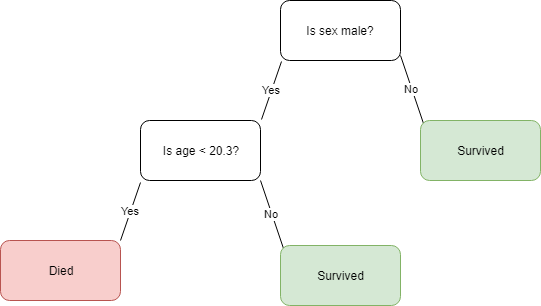
\includegraphics[width=0.8\textwidth]{media/decisiontree_example.png}
	\caption{Example of a decision tree which classifies a passenger to survive a car crash or not.}
	\label{fig:decisiontree_example}
\end{figure}

	%NÄR SKRIVA OM PARAMETRIC: But non-parametric approaches do suffer from a major disadvantage: since they do not reduce the problem of estimating f to a small number of parameters, a very large number of observations (far more than is typically needed for a parametric approach) is required in order to obtain an accurate estimate for f \cite{BOOK:14}.
		Decision tree algorithms are allowed to capture non-linear patterns in the training data, which makes them flexible, but also prone to overfitting \cite{BOOK:7}. Kotiantis \cite{ARTICLE:7} claims that there are two common solutions to battle overfitting in decision tree induction algorithms:
		\begin{enumerate}
			\item Stop the training before it fits the training data perfectly
			\item Prune the decision tree
		\end{enumerate}
		The second method has shown to be more successful in practice than the first one \cite{BOOK:8}. Pruning is a process in which subtrees of the decision tree are replaced by leaves. In other words, the size of the tree is reduced. There are different pruning methods that can be used, but exploring such details are not in the scope of this project.

		 Among several decision tree induction algorithms, CART and C4.5 are the most commonly used \cite{BOOK:8}. CART can solve both regression and classification problems and it is available in Scikit-learn \cite{WEBSITE:16}. %CART can be used to solve multiclass classification problems \cite{ARTICLE:16}
		
	\subsection{Instance based learning} \label{sec:knn}
	Instance-based learning (IBL) algorithms store provided training data, which is used at a later point to predict/classify an observation. In other words, when a new observation is received, an IBL algorithm retrieves related observations from memory and uses them to predict/classify a new observation. This behavior means that IBL algorithms process training data quickly, while the classification/prediction process takes more time when compared to, for example, decision trees \cite{ARTICLE:8}. 

	An example of an IBL algorithm is $k$-Nearest Neighbor (kNN). Generally, observations can be considered to be points in an $n$-dimensional space. The algorithm kNN is based on the principle that observations in a dataset are generally close to other observations with similar properties.  For a new observation, the algorithm finds its $k$ nearest neighbors, and uses the properties of the $k$ nearest neighbors to classify the new observation. kNN can be used to solve both regression and multiclass classification problems in Scikit-learn \cite{WEBSITE:17, WEBSITE:18}.

	Wu et al. \cite{ARTICLE:9} claim that kNN is suitable for multiclass classification problems. Another study by L. Zhong et al. \cite{IP:3} showed success in predicting CT images from MRI data by using kNN regression. However, \cite{ARTICLE:9} mentions that the algorithm is sensitive to the choice of $k$: smaller values can mean it is sensitive to noise and larger values may include too many points from other classes. Overall, Okamoto and Yugami \cite{ARTICLE:12} showed that an optimal choice of $k$ grew linearly with an increase in the amount of training data. This indicates that $k$ should be higher for higher amounts of training data. However, scientific methods for choosing a specific optimal value of $k$ are lacking \cite{ARTICLE:7}.

	Wu et al. \cite{ARTICLE:9} talk about the issues of choosing a distance metric for kNN. They argue that among several choices, it is desirable to have a distance metric in which a smaller value between two nodes implies a stronger connection. Scaling is another factor one needs to consider when using kNN. If one feature $f_1$ varies from, say 1.5 to 1.8, and another $f_2$ from 10,000 to 1,000,000 then $f_2$ will have higher impact on the computation of distance. 
	
	%\subsection{Kernel methods based learning}

	\subsection{Bayesian learning}
		Bayesian algorithms are those that apply the Bayesian inference theorem. This can be used to calculate the probability of a hypothesis $H$ after seeing the data $D$.
		\begin{equation} \label{eq:bayes}
			p(H|D) = \frac{p(H)p(D|H)}{p(D)}
		\end{equation} 
	The basic notion of these kind of algorithms is that classification can be achieved if assumptions can be made from existing data. %Imagine an example of seeing a person whose sex you cannot decide, and you wish to address this person from afar. The person is standing in queue for the men's room, would you call out "excuse me ma'am" or "excuse me sir"? One may assume that this is a man since there is a higher probability of men being in line for the men's room than vice versa. 

	The Naïve bayes algorithm assumes that features in a dataset are independent from one another. This means that each feature contribute independently to classify an observation, regardless of any correlation that might exist among the features, which is why it is called naïve. Naïve bayes is a parametric algorithm due to the fact that it make assumptions on the dataset. Despite its naïve assumption and ease of use, Naïve bayes classifiers have proved successful, even when strong dependencies among features are present \cite{ARTICLE:13, IP:4}. Naïve Bayes can be applied to regression problems through discretization, but it has limited success in comparison to classification problems when the independence assumption does not hold \cite{ARTICLE:14}. Naïve bayes can be applied to multiclass classification problems \cite{ARTICLE:17}. 

	%The Gaussian Naiïve bayes classifier assumes that the features have a gaussian (normal) data distribution.
	 
	\subsection{Regression based learning} \label{sec:reg_based_learning}
		Although the names might be confusing, regression based learning is not the same as regression predictive modelling, whose type of problems are referred to as "regression problems" throughout this project. Regression based learning refers to regression analysis: a number of statistical methods for estimating relationships among variables. This is a well-known tool both in statistics and machine learning. 

		There are three components in a regression model: scalars $\beta_i$, independent variables $X_i$ and dependent variables $Y$. In regression based learning, $X_i$ represent input features, $Y$ is the target feature and $\beta_i$ are parameters which are tuned during the training process. The example shown in equation \ref{eq:example_ws} is an example of a model built with a regression based learning algorithm called Ordinary Least Squares (OLS). OLS can be used to solve regression problems. A regression based learning algorithm called Logistic regression can be used to solve classification problems. 

		Both OLS and Logistic regression are parametric since they make assumptions on the dataset. Some of the assumptions listed by \cite{BOOK:6} that most parametric regression based learning algorithms make:
	\begin{itemize}
		\item{Linear behavior:} If a target feature and an input feature have a linear relationship, they have straight line when plotted against oneanother. Any non-linear relationships between the target feature and other features are assumed to not be used as input features.
		\item{Normal distribution:} Assumes the data of the target feature is normally distributed.
		\item{Outliers:} Are expected to be taken care of.
		\item{Data accuracy:} Values of the target feature that are irrelevant for classification/prediction are assumed to be deleted. For example, error states that are not to be classified are assumed to be deleted.
	\end{itemize} %skriv mer om assumptions?

		Overfitting in regression-based learning algorithms can be thwarted by applying the regularization techniques as seen in section \ref{sec:regularization}. %Feng et. al \cite{ARTICLE:15} chose $\lambda$, which is one of the regularization hyperparameters,  based on which value of $\lambda$ maximised their cross-validation scores. They did so by performing a grid-search (see \ref{sec:hyperparameters}) on $\lambda$. %ex: lambda = e^(x/10), x = -100, -99,...9, 10).http://eds.b.ebscohost.com.proxy.lib.ltu.se/eds/pdfviewer/pdfviewer?vid=6&sid=e3b5f9cf-09c2-4142-81c9-bbfa4b659571@sessionmgr4008

	\subsection{Artificial Neural Networks} \label{sec:deep_learning}
			%Deep learning algorithms are those that aim to learn an artificial neural network (ANN) \cite{BOOK:6}. 
			Artificial Neural Network (ANN) algorithms take inspiration from biological neural networks found in the human brain. An ANN is a directed weighted graph where each node represents an artificial neuron. The graph is organized from left to right by having three type of nodes:
	\begin{itemize}
		\item Input nodes
		\item Hidden layer nodes
		\item Output nodes
	\end{itemize}
			The input nodes are the different input features and the output nodes are possible outcomes. Without going into too much detail, the purpose of the hidden layers is to combine the inputs and project them on a higher dimension. For example, imagine a neural network model trained to recognize triangles. The input nodes represent all of the different pixels. The first hidden layer of that model may distinguish edges in the picture, the second layer recognizes when those edges form complex shapes, and so on. Figure \ref{fig:neuralnetwork_example} depicts an example of an ANN with the same kind of example used to explain how CART works (see figure  \ref{fig:decisiontree_example}).

\begin{figure}[H] 
	\centering
	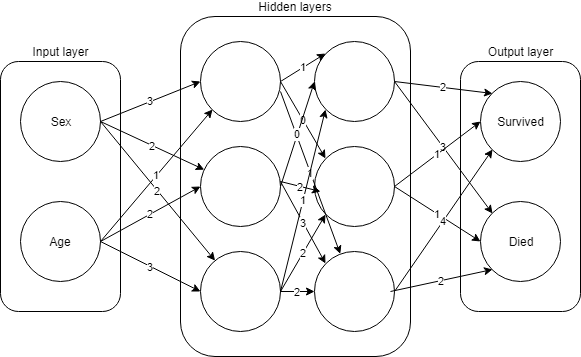
\includegraphics[width=0.8\textwidth]{media/neuralnetwork_ex.png}
	\caption{Example of a neural network with two hidden layers. The goal is to classify if a passenger survives a car crash or not.}
	\label{fig:neuralnetwork_example}
\end{figure}

			The number of hidden layers $h$ and nodes per hidden layer $N_h$ are hyperparameters of ANNs. Hyperparameters are model parameters whose value are set before the training process. So the question one might ask is, what is an good choice for $h$ and $N_h$? Heaton \cite{BOOK:10} writes that having $h=1$ is enough for most practical problems, and that in theory, there is little reason to use more than two hidden layers. As for $N_h$, Heaton writes that a low value of $N_h$ can lead to underfitting whereas the opposite may introduce overfitting and a significant increase in training time. Heaton encourages practitioners to try different values for $N_h$ but provides several rule-of-thumb methods for simplicity, one of which is the following: "The number of hidden neurons should be 2/3 the size of the input layer, plus the size of the output layer". %"The Presence of irrelevant features can make neural network training very inefficient, even impractical" \cite{ARTICLE:7}

			All that's been covered so far of ANNs is the architecture, but how are decisions made? An ANN algorithm known as Multi-layer Perceptron (MLP) is used as an example to explain how choices are made in the ANN: A specific decision is made from the highest valued output node. The value of a specific non-input node is based on an activation function and edge weights from incoming edges. 
%The highest value in the output nodesInputs are processed at input nodes. A non-input node  process input from a node in the previous layer $n_i$ if a node in the previous layer $n_{i-1}$ processed input, and the connecting $E(n_{i-1}, n_{i})$ have the highest weight of all outgoing edges from node $n_{i-1}$. 
A technique known as backpropagation is used in MLP to set the edge weights. In a simple sense, backpropagation updates weights of edges in the ANN based on a loss function. Whenever a classification/prediction is made, the error is propagated backwards in the network from that classification/prediction, and weights are adjusted accordingly. MLP is a supervised learning algorithm that is available in Scikit-learn \cite{WEBSITE:32}.

	\subsection{Ensemble learning}
		Ensemble learning is based on the principle that combining the results of several algorithms into a collective score can produce better results than individual scores. One example of an ensemble learning algorithm Random forest. Random forest averages results from several decision tree classifiers/predictors. Two independent studies indicate that Random forest generally have high performance when compared to other non-ensemble algorithms \cite{ARTICLE:16, IP:5}. Random forest can be applied to classification- and regression problems \cite{WEBSITE:17}

%Chowdhury et. al \cite{ARTICLE:16} conducted a study to see if ensemble methods were superior to CART, kNN, support vector machine and neural network in classifying physical activities. One of the ensemble methods used in the study was Random forest, which showed a constistent high score. Random forest performed second best in an empirical comparison of ten supervised learning algorithms \cite{IP:5}.
		
\section{Generalization} \label{sec:generalization}
	The fundamental goal of machine learning is to generalize beyond observations in the training dataset, since it's unlikely that the same exact observations are found again on unseen data \cite{ARTICLE:3}. Both training error: how well an algorithm performs on its training data, and generalization error: how well a model performs on unseen data, need to be considered in machine learning \cite{BOOK:1}.

	The terminology used to explain how well machine learning models learn and generalize to new data is overfitting and underfitting. They are two central challenges in machine learning \cite{BOOK:1}. 
\begin{itemize}
	\item{Overfitting:} Random fluctuations and statisticical noise is learnt to the extent that it affects the model's ability to generalize. Instead of learning the data trend in the training data, the model "memorizes" it \cite{ARTICLE:4}. An overfit model is overly complex.
	\item{Underfitting:} A model that performs poorly on both its training data and on generalization. An underfit model is too simple.
\end{itemize}

	The goal then, is to select a model that is somewhere between underfitting and overfitting. Underfitting is typically remedied by choosing alternative models, but the most common problem in applied machine learning is how to avoid overfitting \cite{WEBSITE:8}. As a means to check whether or not a model suffers from overfitting, \cite{IP:7} suggests that when the test error of a model exceeds its training error, the model is overfitted to its training data. %however your training error is always lower than your test error. https://nlpers.blogspot.se/2015/09/overfitting.html, lägg till mer källor
According to Davide \cite{ARTICLE:4}  the mere awareness of the issue of overfitting along with two powerful tools: cross-validation and regularization, can be enough to overcome the problem. Feature selection is also brought up in this section as a means to overcome overfitting.

	\subsection{Cross-validation} \label{sec:crossval}
	 An alternative to the holdout approach explained in section \ref{sec:supervisedlearning} is Cross-validation. It is an approach where parts of the data are not necessarily used solely for testing, it can be used for both training and testing. %Although the name might be confusing, the validation is typically done by the test data and a validation dataset is not necessarily used. 
One cross-validation technique is called $k$-fold cross-validation. With this technique, the data is randomly shuffled and split into $k$ folds. The idea is to iterate the training- and test process $k$ times so that every fold has been used once for testing, and ultimately average the performances from $k$ iterations. Using a value of $k = 10$ is a common choice in practice and in which case it is called 10-fold cross-validation \cite{ARTICLE:4}. Furthermore, the results from \cite{BOOK:4} indicate that using $k=10$ is a good choice when it comes to minimizing running-time, limiting bias (underfitting) and variance (overfitting). 

	While this technique can be used to limit overfitting, it also proves useful when dealing with small datasets since all of the data can be used for training \cite{ARTICLE:4}.  On the other hand, a different study shows that since $k$-fold uses its data both for training and evaluation, it isn't entirely unbiased and that it can create naïve models \cite{ARTICLE:25}. %fast är detta bara när man har validation set?


%Cross-validation is an approach where the training data is used for both training and validation.  In cross-validation technique known as $k$-fold cross-validation, the data is randomly split into $k$ folds. The idea is to iterate the training and validation process $k$ times so that every fold has been used once for validation, and ultimately average the performance over $k$ iterations. This eliminates the need of leaving out a subset of the original dataset to be used as a validation dataset. This means that more data can be used for training instead. Using a value of $k = 10$ is a common choice in practice when using $k$-fold cross-validation, and in which case it is called 10-fold cross-validation \cite{ARTICLE:4}. Furthermore, using $k=10$ seems to be optimal when it comes to optimizing run-time for the test, limiting bias (underfitting) and variance (overfitting) \cite{BOOK:4}. By using this technique, the algorithm learns from each subset in the training set and limits the risk of overfitting to the training data \cite{ARTICLE:4}.



	There is a variant of this technique called stratified k-fold cross-validation. In stratified k-fold cross-validation, the folds are created in such a way that each fold contains similar proportions of target features as the full dataset. For example, think of the classification problem of classifying email as spam or not spam. If this technique is applied to the email filtering problem as seen in \ref{sec:classification}, and the ratio of spam/not spam is 20\%/80\% in the original dataset, then the same proportion is attempted to be maintained in each of the $k$ folds. This technique tends to generate less bias and variance when compared to regular k-fold cross validation \cite{IP:2}. It can be applied to regression problems, but the results from Breiman and Spector \cite{ARTICLE:5} indicate that there is little improvement in doing so.

	\subsection{Regularization} \label{sec:regularization}
	Another method used to overcome overfitting is regularization. This technique discourages complexity and flexibility of models by regularizing its coefficients toward zero. The magnitude of the regularization can be controlled by a hyperparameter $\lambda$. The higher value of $\lambda$, the higher impact regularization has on the model. High values on $\lambda$ can result in underfitting and should therefore be controlled carefully \cite{WEBSITE:13}. Three different types of regularization methods:

\begin{itemize}
	\item{$L_1$ regularization (Lasso):} Adds a penalty equal to the sum of the absolute values of $n$ coefficients. This kind of regularization can nullify parameters and for that reason it can be seen as a way to limit the amount of features in the model (see feature selection in \ref{sec:feature_selection}).
		\begin{equation}
			Error_{L_1} = Error + \lambda \sum_{i=1}^{n}|\beta_i| 
		\end{equation}
	\item{$L_2$ regularization (Ridge):} Adds a penalty equal to the sum of the square value of the coefficients. This exhibits a different behavior than $L_1$ regularization in that the coefficients are reduced to zero more slowly.
		\begin{equation}
			Error_{L_2} = Error + \lambda \sum_{i=1}^{n}\beta_i^2 
		\end{equation}
	\item{$L_1/L_2$ regularization (Elastic-net):} A combination of $L_1$ and $L_2$ regularization. A hyperparameter $\alpha$ is set to determine the impact ratio of $L_1$ and $L_2$ regularization, where $0 \leq \alpha \leq 1$.
 		\begin{equation}
			Error_{L_1L_2} = Error + \lambda ( (1-\alpha)\sum_{i=1}^{n}|\beta_i| + \alpha  \sum_{i=1}^{n}\beta_i^2 ) 
		\end{equation}
\end{itemize}

	A comparison of these techniques was made by \cite{ARTICLE:21} in their performance of modelling insulin sensitivity. The results demonstrate a slight advantage to Lasso and Elastic-net in terms of performance. 
%This study examines different regularization approaches to investigate the solution stability of the method of fundamental solutions (MFS). We compare three regularization methods in conjunction with two different regularization parameters to find the optimal stable MFS scheme. Meanwhile, we have investigated the relationship among the condition number, the effective condition number, and the MFS solution accuracy. Numerical results show that the damped singular value decomposition under the parameter choice of the generalized cross-validation performs the best in terms of the MFS stability analysis. We also find that the condition number is a superior criterion to the effective condition number. (C) 2010 IMACS. Published by Elsevier B.V. All rights reserved.

	\subsection{Feature selection} \label{sec:feature_selection}
		Feature selection is a process where irrelevant and redundant features are removed. The curse of dimensionality, which is brought up in section \ref{sec:background}, can be avoided by reducing the amount of input features. Reducing the amount of input features can lead to better generalization and performance \cite{ARTICLE:10, ARTICLE:22}. There are methods in Scikit-learn to perform feature selection based on linear correlation to a model's target feature, removing features with low variance, and more \cite{WEBSITE:30}.
	

%"Feature subset selection is the process of identifying and removing as many irrelevant and redundant features as possible. This reduces the dimensionality of the data and enables data mining algorithms to operate faster and more effectively. The fact that many features depend on one another often unduly influences the accurary of supervised ML classification models. this problem can be addressed by constructing new features from the basic feature set." \cite{ARTICLE:7}
	
	%tip 1 \cite{ARTICLE:4}
	%tip 4, choose simple algorithm \cite{ARTICLE:4}
\section{Optimizing hyperparameters} \label{sec:hyperparameters}
	There exist no solution for finding optimal hyperparameters for machine learning algorithms a priori. Instead, experimentation is needed. One brute-force approach, which according to \cite{BOOK:9} is the best way to find optimized hyperparameters, is to use a technique known as grid search. The technique systematically test hyperparameters incrementally in a given interval. Although the technique may prove useful, it can be computationally intense.

	Another way to test parameters is to use a technique known as random search. As the name suggests, it tests values at random and picks the best choice from a number of random tests. According to \cite{BOOK:9}, this technique works surprisingly well, but the authors recommend to perform at least 15 to 60 tests in order for it to work properly.

\section{Data preparation}
	Data preparation encompass different measures used to update a given dataset. It may involve removing errors, transforming features, scaling features etc. Davide \cite{ARTICLE:4} states that the most important component of a machine learning project is the dataset, and that the success of a machine learning project relies on how the dataset is pre-processed.

	\subsection{Imbalanced data} \label{sec:imbalancedtheory}
	Imbalanced data is covered briefly in section \ref{sec:classification}, in short it means that the classes of a specific feature in a dataset are not equally represented. This may be a concern in classification problems. Fortunately, there are a number of ways to overcome this problem. Davide \cite{ARTICLE:4} suggests that the best way to overcome it is to collect more data. Apart from collecting more data, there is also a method known as oversampling that can be used. The method involves creating new observations from existing ones with underrepresented classes.

	A number of oversampling techniques that can be used to solve multiclass classification problems are suggested by \cite{IP:6}. However the suggested techniques are complex and must be integrated manually to comply with Scikit-learn. Imbalanced-learn is a Scikit-learn compatible Python module that can be used to perform oversampling \cite{WEBSITE:22}. Three techniques are supported for oversampling: Smote, Adasyn and Random oversampler. The techniques can be used to solve multiclass classification problems in Imbalanced-learn, despite not being suggested by \cite{IP:6} as proper techniques to solve such problems. 

	Smote and Adasyn create new synthetic points in the dataset, while Random oversampler creates duplicates. Synthetic points are points that are created from existing points, but with minor adjustments. The disadvantages of using duplicate observations instead of synthetic points is that it introduces overfitting \cite{BOOK:12}. However, both Adasyn and Smote can be configured in a number of ways on how the synthetic points are built, and are therefore not as easy to use as Random oversampler \cite{WEBSITE:23}. 
% tip 5 \cite{ARTICLE:4} https://www.ncbi.nlm.nih.gov/pmc/articles/PMC5721660/
	
	\subsection{Feature engineering}
	Feature engineering concerns manipulation of features in a dataset, in order to attain an overall improved result. Domingos \cite{ARTICLE:3} argues that "feature engineering is the key" in a machine learning project. However, this process can be considered beging more art than science, and as of such, requires human creativity to come up with smart ways to use the given features \cite{BOOK:9}. 

	Apart from choosing proper features, it might also prove useful to scale down a feature, which operates on a different numeric scale than other features in the same dataset. For example, if a dataset feature shows the number of leaves on a tree, this could be up to 30000 during summer-time and zero during the winter. This could be transformed into a discrete and smaller numeric scale having fewer possibilities using the following transformation: 
\begin{align*} 
	& [0, 9999] = \mbox{few} = 0 \\
	& [10000, 19999] = \mbox{medium} = 1 \\
	& [20000, 30000] = \mbox{many} = 2 
\end{align*}
	
	While a simplified representation in this way can be helpful, it can also mean the representation is too simplified. It could be that more classes are needed to represent leaves in the example presented above. For example that three classes isn't enough to capture the characteristics of leaves on a tree, but more classes are needed:
\begin{align*} 
	& [0, 5999] = \mbox{very few} = 0 \\
	& [6000, 11999] = \mbox{few} = 1 \\ 
	& [12000, 17999] = \mbox{medium} = 3 \\
	& [18000, 23999] = \mbox{many} = 4 \\
	& [24000, 30000] = \mbox{very many} = 5 
\end{align*}


% binarization with boosting and oversampling (BBO) oversampling technique proved useful for multiclass classification \cite{ARTICLE:23}

	%https://machinelearningmastery.com/how-to-prepare-data-for-machine-learning/

	%method to filter out noise, outliers http://ieeexplore.ieee.org/stamp/stamp.jsp?tp=&arnumber=6033571

%\end{comment}


\chapter{Method}
Describe what methods are used to carry out the research. Describe that either several machine learning models are used and compared or one is used and the work is to improve it etc.


\section{Research purpose}
\section{Research approach}
\section{Research strategy}


\section{Tools}





\chapter{Implementation and results}
Describe the process of collecting data, training and implementing machine learning algorithms with different methods.

\section{Data collection}

\section{Neural network}
	\subsection{First iteration}
	\subsection{Second iteration}



\chapter{Analysis}
Analyze data from the implementation with respect to the objective of the study.

\section{Neural network}



\chapter{Conclusions and discussion}
\emph{This chapter presents conclusions connected to the aim of this project, as well as an informal discussion on the results obtained.}

\section{Conclusions}
	This aim of this project was to find optimal supervised learning models to model the behavior of three sensors: Optic Eye, Track Ice Road Sensor and DST111. This was desired so that Trafikverket can potentially replace existing sensors to reduce costs, or use as backup in case of failing sensors. The sensors make four different types of measurements in total: precipitation type, precipitation amount, TIRS road surface temperature and DST111 temperature. The objective was broken down into four subtasks which aimed at finding optimal algorithms to model each of the measurements of the sensors.

	The results obtained in this project indicate that the measurements made by Optic Eye: precipitation type and precipitation amount, are best modelled using CART for precipitation type and kNN for precipitation amount. An accuracy score of 0.84 and macro $F1$ score of 0.46 were obtained in modelling precipitation type using Scikit-learn default settings. Precipitation amount was best modelled using kNN, obtaining a performance score $MSE=0.54$ with $k=64$ in Scikit-learn. 

	The two remaining sensors measuring road surface temperature: Track Ice Road Sensor and DST111, were best modelled using Backpropagation and Random forest respectively. Backpropagation was set to use 64 hidden nodes, with which a performance score $MSE=0.88$ was obtained in modelling TIRS road surface temperature. As for modelling DST111 road surface temperature, the best model was obtained by using Random forest on Scikit-learn default settings with a performance score $MSE=10.16$.

\section{Discussion}

	It is up to Trafikverket to decide what a reasonable margin for error is in stating that a model can or cannot model the behavior of a sensor. But when comparing the results from the regression subtasks in this project, DST111 road surface temperature shows a higher error rate than precipitation amount and Track Ice Road Sensor road surface temperature. Since DST111 and TIRS both measure road surface temperature, it is assumed that the model for DST111 generally performs poorly and as of such, the behavior of DST111 is hard to model with the given input features. Since any algorithm which models TIRS in this project can use DST111 road surface temperature as input feature, which proves to have strong linear correlation to TIRS, the author assumes that if TIRS road surface temperature could be used as input feature to model DST111, a better performance could be obtained.

	As for the classification task of classifying precipitation type, the author deems that its performance should be evaluated on its $F1$ score rather than on its accuracy score in this project. The results from \ref{table:classreport_prectype} show that the best model for modelling precipitation type performed well in predicting no precipitation: 90\% while the other precipitation types had significantly lower recall scores, the lowest being rain and snow mixed which was correctly classified in 3\% of its occurrences. The relatively low $F1$ score may be due to the fact that the dataset is imbalanced in terms of precipitation type, and that the imbalanced data problem was not successfully solved in this project. 

	In hindsight, the author thinks that the accumulated performance score presented in \ref{sec:method_results} can be improved by not allowing negative values in the overfitting score. An overfitting score of 0 means that the model performs equally well on both the training and test dataset. A negative overfitting score means a model performed better on the test dataset than on its training dataset. The author suspects that a negative overfitting score is not necessarily better than one around zero, but a negative overfitting score have a positive impact on the accumulated performance score. This may result in non-optimal algorithms having higher accumulated performance scores than optimal ones, and thus being identified as top performers.

\section{Recommendations}
		The author recommends Trafikverket to refrain from modelling DST111 road surface temperature using the given algorithm and algorithm settings, but to investigate the possibility of modelling Track Ice Road Sensor road surface temperature and precipitation amount using the algorithms and algorithm settings seen in \ref{table:results_summary}. Given that all precipitation types are equally important to classify, the author recommends Trafikverket to investigate if the imbalanced data problem of precipitation type can be solved, either by collecting more data from the less represented classes, or to see if the problem can be solved using similar techniques as the ones used in this project (see attempts in handling class imbalance in \ref{sec:class_imbalance}). 

\chapter{Discussion}

\section{Thesis process}

\section{Validity & Reliability}

\section{Suggestions for future studies}



\end{document}
